\documentclass[aspectratio=169,10pt]{beamer}

\usetheme{Madrid}
\setbeamertemplate{navigation symbols}{}
\setbeamertemplate{footline}[frame number]

\usepackage{amsmath}
\usepackage{amssymb}
\usepackage{array}
\usepackage{booktabs}
\usepackage{graphicx}
\usepackage{tabularx}
\usepackage{tikz}
\usetikzlibrary{arrows.meta,calc,positioning}

\graphicspath{{../data/}{../figures/}}

\definecolor{LectureBlue}{RGB}{13,76,100}
\definecolor{LectureTeal}{RGB}{0,118,122}
\definecolor{LectureGold}{RGB}{194,142,37}
\definecolor{Slate}{RGB}{58,68,84}
\definecolor{SoftGray}{RGB}{245,247,249}

\setbeamercolor{title}{fg=LectureBlue}
\setbeamercolor{subtitle}{fg=Slate}
\setbeamercolor{frametitle}{fg=LectureBlue,bg=LectureBlue!8}
\setbeamercolor{structure}{fg=LectureBlue}
\setbeamercolor{block title}{fg=white,bg=LectureBlue}
\setbeamercolor{block body}{fg=black,bg=SoftGray}
\setbeamercolor{alerted text}{fg=LectureGold}

\renewcommand{\arraystretch}{1.12}

\title{Digital Image Representation, Geometry, and Resampling}
\author{}
\date{May 2026}

\begin{document}

\begin{frame}[plain]
\begin{columns}[c,onlytextwidth]
\column{0.58\textwidth}
{\usebeamerfont{title}\color{LectureBlue}\inserttitle\par}
\vspace{0.4em}
{\usebeamerfont{subtitle}\color{Slate}\insertsubtitle\par}

{\small \insertauthor \hfill \insertdate}

\column{0.38\textwidth}
\includegraphics[width=\linewidth]{ct.jpeg}
\end{columns}
\end{frame}

\begin{frame}{Contents}

\begin{itemize}
\item Digital image formation as a sequence of operators
\item Sampling, quantization, and geometric resampling as information-processing steps
\item Coordinate systems, transform models, and interpolation
\item Why these classical choices still matter in deep learning
\end{itemize}



\end{frame}

\begin{frame}
\begin{center}
  
\includegraphics[height=1\textheight]{../figures/sampling_quantile.png}

\end{center}

\end{frame}




\begin{frame}{Image processing as a Operator}
\begin{columns}[T,onlytextwidth]
\column{0.58\textwidth}
\[
\mathbf{y} = Q\Bigl(S\bigl(h * g\bigr) \Bigr)
\]
\vspace{-0.5em}
\begin{itemize}
\item $g$: underlying continuous scene or object
\item $h$: imaging blur or point-spread function or some filtering operation
\item $S$: spatial sampling operator
\item $Q$: quantization to a discrete numeric representation
\end{itemize}


\column{0.37\textwidth}
\centering
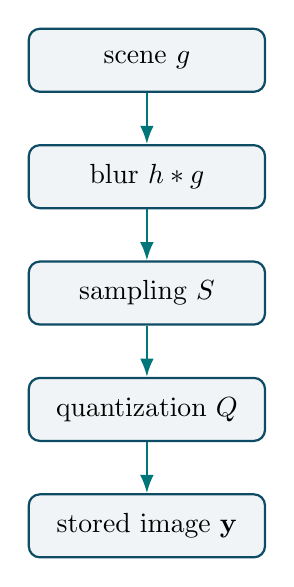
\begin{tikzpicture}[node distance=0.65cm,>=Latex]
\tikzstyle{stage}=[draw=LectureBlue,rounded corners,thick,minimum width=3.0cm,minimum height=0.8cm,fill=LectureBlue!6]
\node[stage] (scene) {scene $g$};
\node[stage,below=of scene] (blur) {blur $h*g$};
\node[stage,below=of blur] (sample) {sampling $S$};
\node[stage,below=of sample] (quantize) {quantization $Q$};
\node[stage,below=of quantize] (image) {stored image $\mathbf{y}$};
\draw[->,thick,LectureTeal] (scene) -- (blur);
\draw[->,thick,LectureTeal] (blur) -- (sample);
\draw[->,thick,LectureTeal] (sample) -- (quantize);
\draw[->,thick,LectureTeal] (quantize) -- (image);
\end{tikzpicture}
\end{columns}
\end{frame}



\begin{frame}{Sampling as an Operator}
\begin{columns}[T,onlytextwidth]
\column{0.56\textwidth}
\[
g_s(x,y) = g(x,y) \sum_{m,n \in \mathbb{Z}} \delta(x-m\Delta_x)\delta(y-n\Delta_y)
\]
\vspace{-0.5em}
\begin{itemize}
\item Sampling is multiplication by a spatial impulse train.
\item In the frequency domain, this produces replicated spectra.
\item If replicas overlap, aliasing occurs and the overlap cannot be undone from the sampled image alone.
\end{itemize}

\begin{block}{Animation}
https://phiresky.github.io/convolution-demo/
\end{block}

\column{0.40\textwidth}
\centering
\begin{center}
  
\includegraphics[width=0.8\linewidth]{../figures/sampling.png}

\end{center}
\end{columns}
\end{frame}

\begin{frame}{Nyquist, Aliasing, and the Cost of Undersampling}
\begin{columns}[T,onlytextwidth]
\column{0.55\textwidth}
\begin{itemize}
\item Smaller pixel spacing permits higher recoverable spatial frequency.
\item A classical bound is $\Delta_x \leq 1/(2B_x)$ and $\Delta_y \leq 1/(2B_y)$ for scene bandwidths $B_x, B_y$.
\item Downsampling without prefiltering folds high frequencies into lower frequencies.
\item In scientific imaging, aliasing corrupts measurement, not just aesthetics.
\end{itemize}
\vspace{0.5em}
\begin{block}{}
Sample at least twice as fast as the highest spatial frequency you want to preserve, or suppress that frequency before sampling.
\end{block}

\column{0.40\textwidth}
\centering
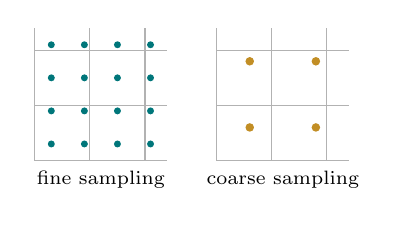
\begin{tikzpicture}[scale=0.7]
\draw[gray!60] (0,0) grid (2.4,2.4);
\foreach \x in {0.3,0.9,1.5,2.1}
  \foreach \y in {0.3,0.9,1.5,2.1}
    \fill[LectureTeal] (\x,\y) circle (1.8pt);
\node[font=\scriptsize] at (1.2,-0.35) {fine sampling};

\begin{scope}[xshift=3.3cm]
\draw[gray!60] (0,0) grid (2.4,2.4);
\foreach \x in {0.6,1.8}
  \foreach \y in {0.6,1.8}
    \fill[LectureGold] (\x,\y) circle (2.2pt);
\node[font=\scriptsize] at (1.2,-0.35) {coarse sampling};
\end{scope}
\end{tikzpicture}
\vspace{0.2em}

\includegraphics[height=0.23\textheight]{ct.jpeg}
\end{columns}
\end{frame}

\begin{frame}{Resolution Is Not the Same as Pixel Count}
\begin{columns}[T,onlytextwidth]
\column{0.52\textwidth}
\begin{itemize}
\item Pixel count is a grid property; resolution is an effective ability to distinguish nearby structure.
\item Optical blur, detector blur, motion blur, and reconstruction kernels all affect effective resolution.
\item Partial-volume effects arise when one voxel contains multiple tissue types or materials.
\item A finely sampled but strongly blurred image can still have poor effective resolution.
\end{itemize}

\begin{block}{Research implication}
Do not infer resolving power from image size alone. The point-spread function matters.
\end{block}

\column{0.42\textwidth}
\small
\begin{tabularx}{\linewidth}{>{\bfseries}p{0.34\linewidth} X}
\toprule
Quantity & What it controls \\
\midrule
Pixel spacing & sampling grid \\
Field of view & spatial coverage \\
Point-spread function & effective blur \\
Slice thickness & through-plane averaging \\
\bottomrule
\end{tabularx}
\end{columns}
\end{frame}

\begin{frame}{Quantization Sets Intensity Resolution}

\begin{itemize}
\item Quantization maps a continuous intensity range to a finite set of gray levels.
\item An 8-bit image stores $2^8 = 256$ levels; a 12-bit image stores 4096 levels.
\item Too few levels create banding, contouring, or loss of subtle contrast.
\item Acquisition depth and display depth are not always the same: CT often stores more precision than we display at once.
\end{itemize}


\end{frame}


\begin{frame}{Information Loss and Invertibility}
\small
\begin{tabularx}{\textwidth}{>{\bfseries}p{0.2\textwidth} >{\raggedright\arraybackslash}p{0.22\textwidth} X}
\toprule
Operation & Invertible? & Reason \\
\midrule
Translation on an infinite grid & Often yes & It rearranges coordinates without collapsing distinct values. \\
Rotation plus interpolation & Approximate only & Interpolation introduces model-based approximation and boundary loss. \\
Downsampling & No & Multiple high-resolution images map to the same coarse image. \\
Quantization & No & Continuous intensity intervals collapse to the same stored value. \\
Cropping & No & Discarded spatial support is unavailable later. \\
\bottomrule
\end{tabularx}


\end{frame}

\begin{frame}{Common Artifacts From Poor Discretization}
\small
\begin{tabularx}{\textwidth}{>{\bfseries}p{0.23\textwidth} X}
\toprule
Artifact & Interpretation \\
\midrule
Aliasing & Sampling is too coarse for the spatial detail in the scene. Fine texture can appear as false low-frequency patterns. \\
Banding & Quantization is too coarse, so smooth intensity transitions become step-like. \\
Interpolation blur & Repeated resampling smooths edges and attenuates high-frequency information. \\
Broken labels & Using linear or cubic interpolation on masks creates invalid class values between labels. \\
\bottomrule
\end{tabularx}

\end{frame}

\begin{frame}{Coordinate Systems Matter}
\begin{columns}[T,onlytextwidth]
\column{0.50\textwidth}
\begin{itemize}
\item \textbf{Index space}: array coordinates such as $(i,j,k)$.
\item \textbf{Physical space}: coordinates measured in mm or another physical unit.
\end{itemize}


\column{0.44\textwidth}
\[
\mathbf{x}_{\mathrm{phys}} = D\,\mathbf{x}_{\mathrm{idx}} + \mathbf{o}
\]
\vspace{-0.5em}
\begin{itemize}
\item $D$: spacing and orientation
\item $\mathbf{o}$: origin
\end{itemize}
\end{columns}
\end{frame}

\begin{frame}{Geometric Transforms: What Changes and What Stays}
\small
\begin{tabularx}{\textwidth}{>{\bfseries}p{0.15\textwidth} >{\raggedright\arraybackslash}p{0.24\textwidth} >{\raggedright\arraybackslash}p{0.22\textwidth} X}
\toprule
Family & Form & Preserves & Typical use \\
\midrule
Rigid & $\mathbf{x}' = R\mathbf{x} + \mathbf{t}$ & distance and angle & translation and rotation \\
Similarity & $\mathbf{x}' = sR\mathbf{x} + \mathbf{t}$ & angle and overall shape & zoom plus rigid motion \\
Affine & $\mathbf{x}' = A\mathbf{x} + \mathbf{t}$ & straight lines and parallelism & scale, shear, skew \\
Projective & $\tilde{\mathbf{x}}' = H\tilde{\mathbf{x}}$ & straight lines & perspective correction, camera-plane mapping \\
\bottomrule
\end{tabularx}

\vspace{0.6em}
\begin{block}{Key idea}
The transform changes coordinates first. Intensity values are assigned only after we decide where the new sample locations lie.
\end{block}
\end{frame}

\begin{frame}{Homogeneous Coordinates Make Composition Clean}
\begin{columns}[T,onlytextwidth]
\column{0.58\textwidth}
\[
\tilde{\mathbf{x}} = \begin{bmatrix}x \\ y \\ 1\end{bmatrix}, \qquad
\tilde{\mathbf{x}}' =
\begin{bmatrix}
a_{11} & a_{12} & t_x \\
a_{21} & a_{22} & t_y \\
0 & 0 & 1
\end{bmatrix}
\tilde{\mathbf{x}}
\]
\vspace{-0.5em}
\begin{itemize}
\item Translation becomes part of one matrix multiplication.
\item Composition is matrix multiplication, which simplifies software and theory.
\item Projective transforms generalize this idea by allowing a nontrivial last row.
\end{itemize}

\column{0.36\textwidth}
\begin{block}{Key gain}
Homogeneous coordinates turn geometric bookkeeping into linear algebra.
\end{block}
\end{columns}
\end{frame}

\begin{frame}{Geometric Intuition: A Camera View Is Already a Transform}
\begin{columns}[T,onlytextwidth]
\column{0.48\textwidth}
\includegraphics[height=0.36\textheight]{book.jpg}

\column{0.48\textwidth}
\includegraphics[height=0.36\textheight]{moving_book.jpg}
\end{columns}

\vspace{0.2em}
\small
\begin{block}{Interpretation}
Even before registration is discussed, perspective changes, viewpoint shifts, and cropping already imply a geometric transform between two images of the same object.
\end{block}
\end{frame}

\begin{frame}{Forward Mapping Versus Backward Mapping}
\begin{columns}[T,onlytextwidth]
\column{0.52\textwidth}
\[
I_{\mathrm{out}}(\mathbf{x}') = I_{\mathrm{in}}\bigl(T^{-1}(\mathbf{x}')\bigr)
\]
\vspace{-0.6em}
\begin{itemize}
\item Forward mapping pushes pixels from input to output and can leave holes.
\item Backward mapping loops over the output grid and asks: where did this location come from in the input image?
\item Because $T^{-1}(\mathbf{x}')$ is usually not on an exact pixel center, interpolation is required.
\end{itemize}

\begin{block}{Why this matters}
Most practical libraries resample with backward mapping because it guarantees that every output pixel is addressed.
\end{block}

\column{0.44\textwidth}
\centering
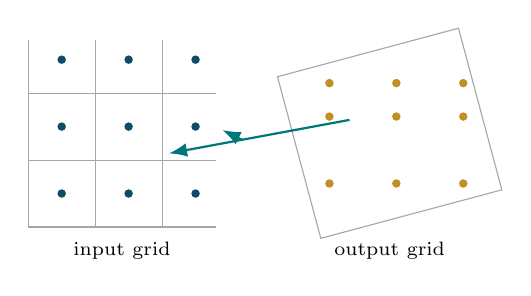
\begin{tikzpicture}[>=Latex,scale=0.85]
\draw[gray!70] (0,0) grid (2.8,2.8);
\foreach \x in {0.5,1.5,2.5}
  \foreach \y in {0.5,1.5,2.5}
    \fill[LectureBlue] (\x,\y) circle (1.8pt);
\node[font=\scriptsize] at (1.4,-0.35) {input grid};

\begin{scope}[xshift=4.0cm,yshift=0.15cm]
\draw[gray!70,rotate around={15:(1.4,1.25)}] (0,0) rectangle (2.8,2.5);
\foreach \x in {0.5,1.5,2.5}
  \foreach \y in {0.5,1.5,2.0}
    \fill[LectureGold] (\x,\y) circle (1.8pt);
\node[font=\scriptsize] at (1.4,-0.50) {output grid};
\end{scope}

\draw[->,thick,LectureTeal] (3.2,1.3) -- (2.9,1.45);
\draw[->,thick,LectureTeal] (4.8,1.6) -- (2.1,1.1);
\end{tikzpicture}
\end{columns}
\end{frame}

\begin{frame}{Interpolation as a Kernel Model}
\begin{columns}[T,onlytextwidth]
\column{0.58\textwidth}
\[
I(x,y) = \sum_{m,n} I[m,n] \, \phi(x-m)\,\phi(y-n)
\]
\vspace{-0.6em}
\begin{itemize}
\item Interpolation is a choice of basis or kernel $\phi$ on the discrete grid.
\item Nearest neighbor uses a box-like basis.
\item Bilinear uses a triangular basis.
\item Cubic methods use smoother kernels with wider support.
\end{itemize}

\begin{block}{Advanced viewpoint}
Interpolation is not merely filling gaps. It imposes an assumption about the class of continuous functions consistent with the sampled data.
\end{block}

\column{0.36\textwidth}
\centering
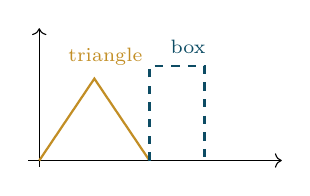
\begin{tikzpicture}[x=0.7cm,y=0.8cm]
\draw[->] (-0.2,0) -- (4.4,0);
\draw[->] (0,-0.1) -- (0,2.1);
\draw[LectureGold,thick] (0,0) -- (1,1.3) -- (2,0);
\draw[LectureBlue,thick,dashed] (2,0) -- (2,1.5) -- (3,1.5) -- (3,0);
\node[font=\scriptsize,LectureGold] at (1.2,1.65) {triangle};
\node[font=\scriptsize,LectureBlue] at (2.7,1.8) {box};
\end{tikzpicture}
\end{columns}
\end{frame}

\begin{frame}{Interpolation Choices}
\small
\begin{tabularx}{\textwidth}{>{\bfseries}p{0.17\textwidth} >{\raggedright\arraybackslash}p{0.15\textwidth} >{\raggedright\arraybackslash}p{0.23\textwidth} X}
\toprule
Method & Support & Strengths & Use with care \\
\midrule
Nearest neighbor & 1 sample & preserves labels exactly, fastest & blocky edges in intensity images \\
Bilinear & $2 \times 2$ neighborhood & stable default for many intensity images & slight blur after repeated use \\
Bicubic & $4 \times 4$ neighborhood & smoother appearance, better edge continuity & can ring near sharp transitions \\
Spline / higher order & larger support & smooth derivatives, useful in scientific resampling & more computation and stronger assumptions \\
\bottomrule
\end{tabularx}

\vspace{0.6em}
\begin{alertblock}{Golden rule}
Intensity images and segmentation masks should almost never be resampled with the same interpolation rule.
\end{alertblock}
\end{frame}

\begin{frame}{Bilinear Interpolation Written Explicitly}
\small
Suppose $(x,y)$ lies inside the cell with corner intensities $I_{00}, I_{10}, I_{01}, I_{11}$ and local coordinates $\alpha, \beta \in [0,1]$.

\[
I(x,y) = (1-\alpha)(1-\beta)I_{00} + \alpha(1-\beta)I_{10} + (1-\alpha)\beta I_{01} + \alpha\beta I_{11}
\]

\begin{itemize}
\item The weights sum to one, so constants are preserved.
\item The estimate is linear along each axis, but repeated use still smooths high-frequency detail.
\item For differentiable image warping, this formula is attractive because gradients are simple almost everywhere.
\end{itemize}
\end{frame}

\begin{frame}{Interpolation Has a Spectral Interpretation}
\begin{columns}[T,onlytextwidth]
\column{0.53\textwidth}
\begin{itemize}
\item Every interpolation kernel has a transfer function in frequency.
\item Nearest neighbor preserves edges aggressively but leaks high-frequency artifacts.
\item Bilinear is smoother but attenuates high frequencies more strongly.
\item Higher-order kernels can better preserve smooth structure but may introduce ringing.
\end{itemize}

\begin{block}{Why this slide is here}
We are not doing a full Fourier lecture, but PhD students should know that interpolation is a filtering decision in disguise.
\end{block}

\column{0.41\textwidth}
\centering
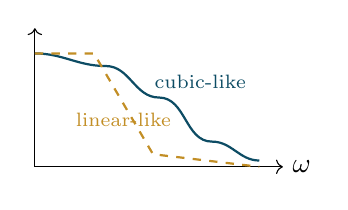
\begin{tikzpicture}[x=0.75cm,y=0.8cm]
\draw[->] (0,0) -- (4.2,0) node[right] {$\omega$};
\draw[->] (0,0) -- (0,2.2);
\draw[LectureBlue,thick] (0,1.8) to[out=0,in=180] (1.2,1.6) to[out=0,in=180] (2.1,1.1) to[out=0,in=180] (3.0,0.4) to[out=0,in=180] (3.8,0.1);
\draw[LectureGold,thick,dashed] (0,1.8) -- (1.0,1.8) -- (2.0,0.2) -- (3.8,0.0);
\node[font=\scriptsize,LectureBlue] at (2.8,1.35) {cubic-like};
\node[font=\scriptsize,LectureGold] at (1.5,0.75) {linear-like};
\end{tikzpicture}
\end{columns}
\end{frame}

\begin{frame}{Boundary Conditions and Repeated Resampling}
\begin{columns}[T,onlytextwidth]
\column{0.52\textwidth}
\begin{itemize}
\item Outside-image values must be defined: zero padding, border replication, reflection, or periodic wrap.
\item Boundary choices change local statistics and may create artifacts near the image edge.
\item Repeated interpolation compounds smoothing and can slowly drift geometry.
\end{itemize}

\begin{block}{Best practice}
Compose geometric transforms first and resample once whenever possible.
\end{block}

\column{0.42\textwidth}
\small
\begin{tabularx}{\linewidth}{>{\bfseries}p{0.33\linewidth} X}
\toprule
Rule & Consequence \\
\midrule
Zero pad & dark halo risk \\
Replicate & flat edges \\
Reflect & often visually stable \\
Wrap & rarely physical in imaging \\
\bottomrule
\end{tabularx}
\end{columns}
\end{frame}

\begin{frame}{Labels Are Not Intensities}
\begin{columns}[T,onlytextwidth]
\column{0.50\textwidth}
\begin{itemize}
\item A grayscale image encodes ordered numeric intensity.
\item A segmentation mask encodes categorical identity.
\item Linear interpolation between labels 1 and 3 producing 2 is usually meaningless.
\end{itemize}

\column{0.44\textwidth}
\small
\begin{tabularx}{\linewidth}{>{\bfseries}p{0.35\linewidth} X}
\toprule
Data type & Typical interpolation \\
\midrule
Intensity image & linear or cubic \\
Label map & nearest neighbor \\
\bottomrule
\end{tabularx}
\end{columns}
\end{frame}

\begin{frame}{3D Images Add Another Layer of Difficulty}
\begin{columns}[T,onlytextwidth]
\column{0.54\textwidth}
\begin{itemize}
\item Many volumetric datasets are anisotropic: in-plane spacing differs from through-plane spacing.
\item Resampling to isotropic voxels can simplify analysis, but the through-plane direction may contain less true information.
\item Thin-slice and thick-slice data should not be treated as equivalent just because arrays are resampled to the same shape.
\end{itemize}

\begin{block}{Practical warning}
Resampling can standardize geometry, but it cannot create missing anatomical detail along poorly sampled directions.
\end{block}

\column{0.40\textwidth}
\[
\Delta_x \neq \Delta_y \neq \Delta_z
\]
\vspace{-0.4em}
\begin{itemize}
\item voxel shape matters
\item slice thickness matters
\item metadata matters
\end{itemize}
\end{columns}
\end{frame}

\begin{frame}{A Practical Resampling Checklist}
\begin{columns}[T,onlytextwidth]
\column{0.49\textwidth}
\begin{block}{Before resampling}
\begin{itemize}
\item Define the reference grid: size, spacing, origin, and orientation.
\item Decide whether the task is visualization, measurement, or model input preparation.
\item Use anti-alias filtering before aggressive downsampling.
\end{itemize}
\end{block}

\column{0.49\textwidth}
\begin{block}{During resampling}
\begin{itemize}
\item Use backward mapping.
\item Choose interpolation that matches the data type.
\item Track geometry metadata so physical distances remain meaningful.
\end{itemize}
\end{block}
\end{columns}

\vspace{0.6em}
\begin{alertblock}{Common mistake}
Changing image size without updating pixel spacing creates visually plausible images that are geometrically wrong.
\end{alertblock}
\end{frame}

\begin{frame}{Discussion Checkpoint}
\begin{block}{Think before the break}
You receive multi-site CT images with different spacings, reconstruction kernels, and intensity ranges. You want to train one model across all sites.
\end{block}

\vspace{0.5em}
\begin{enumerate}
\item Which differences should be normalized by preprocessing?
\item Which differences reflect genuine information loss rather than nuisance variation?
\item Which choices risk making the model easier to train but less scientifically valid?
\end{enumerate}
\end{frame}

\begin{frame}{Deep Learning Still Depends on Classical Image Manipulation}
\begin{columns}[T,onlytextwidth]
\column{0.32\textwidth}
\begin{block}{Preprocessing}
\begin{itemize}
\item resize or crop to fixed input shapes
\item normalize intensity after choosing a display or physical range
\item standardize spacing across scanners or sites
\end{itemize}
\end{block}

\column{0.32\textwidth}
\begin{block}{Augmentation}
\begin{itemize}
\item flips, rotations, zoom, and elastic warps
\item label geometry must follow the image exactly
\item augmentation cannot recover detail lost by undersampling
\end{itemize}
\end{block}

\column{0.32\textwidth}
\begin{block}{Learnable geometry}
\begin{itemize}
\item Spatial Transformer Networks predict a warp and then resample differentiably
\item the grid sampler is classical interpolation inside a neural network
\item modern models still inherit the same resampling trade-offs
\end{itemize}
\end{block}
\end{columns}
\end{frame}

\begin{frame}{Differentiable Resampling Inside Neural Networks}
\small
Spatial Transformer Networks use a learned transform and a differentiable sampler. For bilinear sampling,

\[
V_i^c = \sum_n \sum_m U_{nm}^c \max(0,1-|x_i^s-m|)\max(0,1-|y_i^s-n|)
\]

\begin{itemize}
\item $U$: input feature map, $V$: output feature map
\item $(x_i^s, y_i^s)$: sampled source coordinate predicted by the network
\item The sampler is modern deep learning built on classical interpolation
\end{itemize}

\begin{alertblock}{Important perspective}
Neural networks can learn where to sample, but they still inherit the mathematical biases of the interpolation kernel.
\end{alertblock}
\end{frame}

\begin{frame}{Learned Upsampling Does Not Nullify Sampling Theory}
\begin{columns}[T,onlytextwidth]
\column{0.52\textwidth}
\begin{itemize}
\item Super-resolution can produce plausible high-frequency content by using learned priors.
\item This is not the same as recovering the exact pre-sampled signal.
\item For scientific or medical tasks, visually convincing hallucination may be harmful.
\end{itemize}

\begin{block}{PhD-level distinction}
There is a difference between perceptual realism, statistical plausibility, and faithful recovery of the original scene.
\end{block}

\column{0.42\textwidth}
\begin{alertblock}{Ask this in papers}
Is the method optimizing appearance, downstream prediction, or physical fidelity?
\end{alertblock}
\end{columns}
\end{frame}

\begin{frame}{Augmentation Is Geometry Plus Assumption}
\begin{columns}[T,onlytextwidth]
\column{0.50\textwidth}
\begin{itemize}
\item Rotations, flips, elastic warps, and crops encode beliefs about nuisance variation.
\item If the augmentation violates the acquisition process or anatomy, the model learns unrealistic invariances.
\item For labels, every augmentation rule must be mirrored by a compatible label transform.
\end{itemize}

\column{0.44\textwidth}
\begin{block}{Good augmentation asks}
Which transformations preserve the task label in the real world?
\end{block}

\begin{alertblock}{Bad augmentation asks}
What can we randomize because the library supports it?
\end{alertblock}
\end{columns}
\end{frame}

\begin{frame}{Example Workflow: CT Scan to Model Input}
\begin{columns}[T,onlytextwidth]
\column{0.35\textwidth}
\includegraphics[width=\linewidth]{ct.jpeg}

\column{0.61\textwidth}
\begin{enumerate}
\item Start from the acquired scanner grid with its own spacing and intensity precision.
\item Resample to a common target spacing so anatomy has a consistent physical scale.
\item Window or normalize intensities for the downstream task.
\item Crop or pad to the model input size.
\item If labels exist, transform them with the same geometry but nearest-neighbor interpolation.
\end{enumerate}

\vspace{0.5em}
\begin{block}{Interpretation}
The network never sees the original scene directly. It sees a sampled, quantized, and resampled tensor whose quality depends on all earlier design choices.
\end{block}
\end{columns}
\end{frame}

\begin{frame}{Failure Modes in Machine-Learning Pipelines}
\small
\begin{tabularx}{\textwidth}{>{\bfseries}p{0.28\textwidth} X}
\toprule
Failure mode & Consequence \\
\midrule
Resizing all images to one shape without respecting spacing & anatomy appears at inconsistent physical scales \\
Linear interpolation on masks & invalid labels and boundary corruption \\
Repeated random resampling in data loading & hidden blur and train-test mismatch \\
Aggressive windowing before analysis & loss of subtle intensity structure \\
Ignoring acquisition blur differences across scanners & site-specific artifacts masquerade as biological signal \\
\bottomrule
\end{tabularx}
\end{frame}

\begin{frame}{Seminar Prompt}
\begin{block}{A good research question}
When a model trained on one imaging protocol fails on another, how much of the error is due to representation mismatch rather than model capacity?
\end{block}

\vspace{0.6em}
\begin{itemize}
\item What would you standardize?
\item What would you leave untouched to preserve scientific validity?
\item How would you design an ablation to separate geometry effects from model effects?
\end{itemize}
\end{frame}

\begin{frame}{Take-Home Messages}
\begin{itemize}
\item A digital image is the output of an acquisition model, not a neutral copy of reality.
\item Sampling, blur, quantization, cropping, and resampling each impose distinct information limits.
\item Geometry requires explicit coordinate reasoning; array shape alone is not enough.
\item Interpolation is a modeling choice with spatial, spectral, and statistical consequences.
\item Deep-learning pipelines still rest on these classical decisions, even when the warping is differentiable or learned.
\end{itemize}
\end{frame}

\begin{frame}{Suggested Reading}
\small
\begin{itemize}
\item R. C. Gonzalez and R. E. Woods, \emph{Digital Image Processing}, 3rd ed.
\item R. Szeliski, \emph{Computer Vision: Algorithms and Applications}, 2nd ed.
\item M. Jaderberg et al., \emph{Spatial Transformer Networks}, NeurIPS 2015.
\item J. A. Fessler, \emph{Fundamentals of Image Reconstruction}, for a stronger operator viewpoint.
\end{itemize}

\vspace{1em}
\begin{block}{Final discussion prompt}
If a model input must be resized from $512 \times 512$ to $224 \times 224$, which information is lost, which information can be partially approximated by a model, and which scientific claims become harder to justify afterward?
\end{block}
\end{frame}

\end{document}
